\begin{figure*}[!t]
  \centering
  \includegraphics[width=0.93\textwidth]{active_trajectory.png}
  \caption{Sparse training cameras and the virtual views chosen for restoration. Each panel projects camera centers into its first two principal axes and uses its own scale. The active planner reranks candidates with the updated scene's alpha maps in round two.}
  \label{fig:active_trajectory}
\end{figure*}

\begin{figure*}[!t]
  \centering
  \includegraphics[width=0.93\textwidth]{closed_loop_psnr.png}
  \caption{Held-out PSNR change from the initial sparse model at each round. The panels use independent vertical ranges to show within-scene differences.}
  \label{fig:closed_loop}
\end{figure*}

\begin{figure*}[!t]
  \centering
  \includegraphics[width=0.93\textwidth]{pseudo_views.png}
  \caption{Two Re10k-1 virtual views before and after reference-guided diffusion, selected for highest verified support in round one and lowest verified support in round two. Each reference is a real sparse training view. The confidence map shows the pixel weights used by gated fusion.}
  \label{fig:pseudo_views}
\end{figure*}

\begin{figure*}[!t]
  \centering
  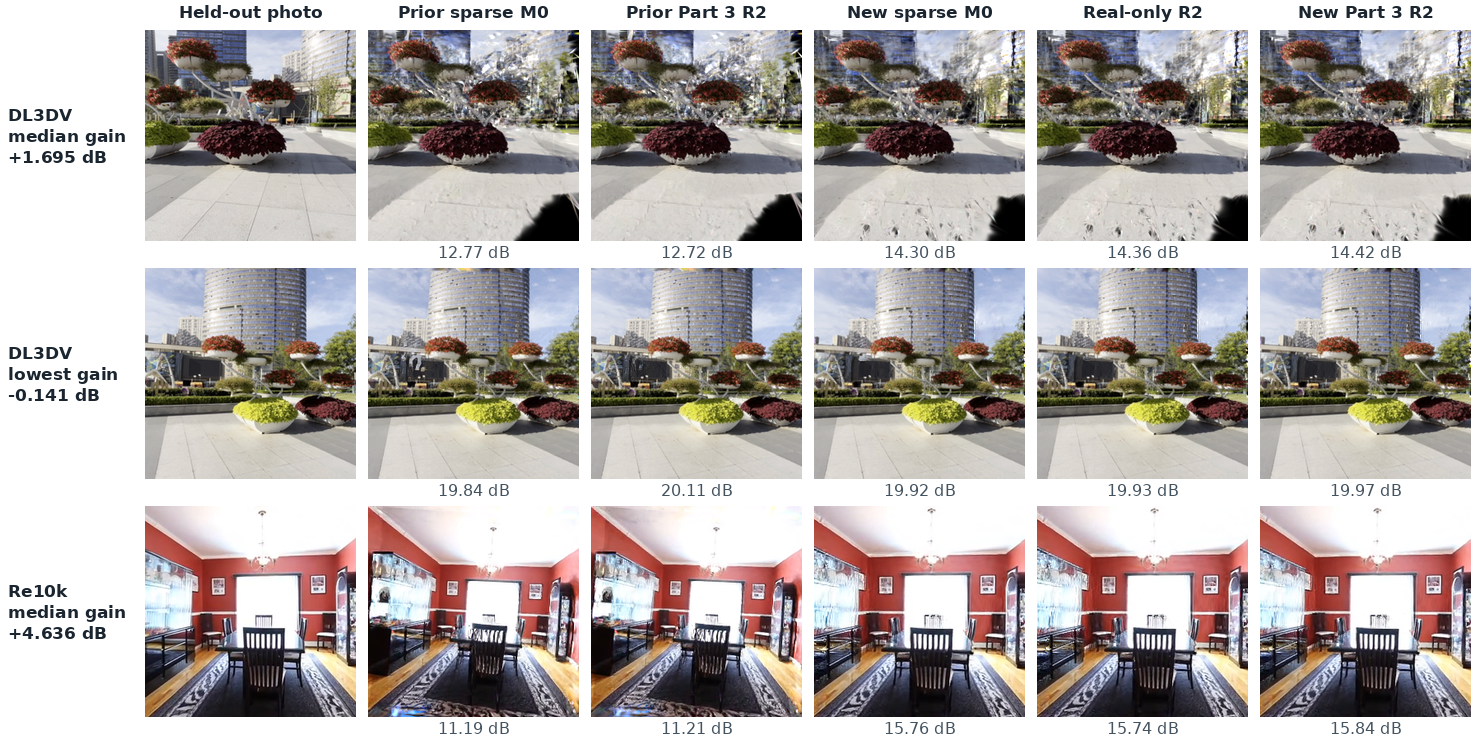
\includegraphics[width=0.93\textwidth]{../results/part3_mse30/heldout_comparison.png}
  \caption{Raw renders from the 13k texture-guided study at matched held-out viewpoints. Rows show the median and lowest PSNR gains on DL3DV and the median gain on Re10k relative to the earlier Part~3 result. The real-only column uses the same initialization and extra training budget.}
  \label{fig:loop_qual}
\end{figure*}
